\section{Plant considered for system identification} \label{sec:plant_considered}
    
    \begin{figure}[htb]
        \centering
        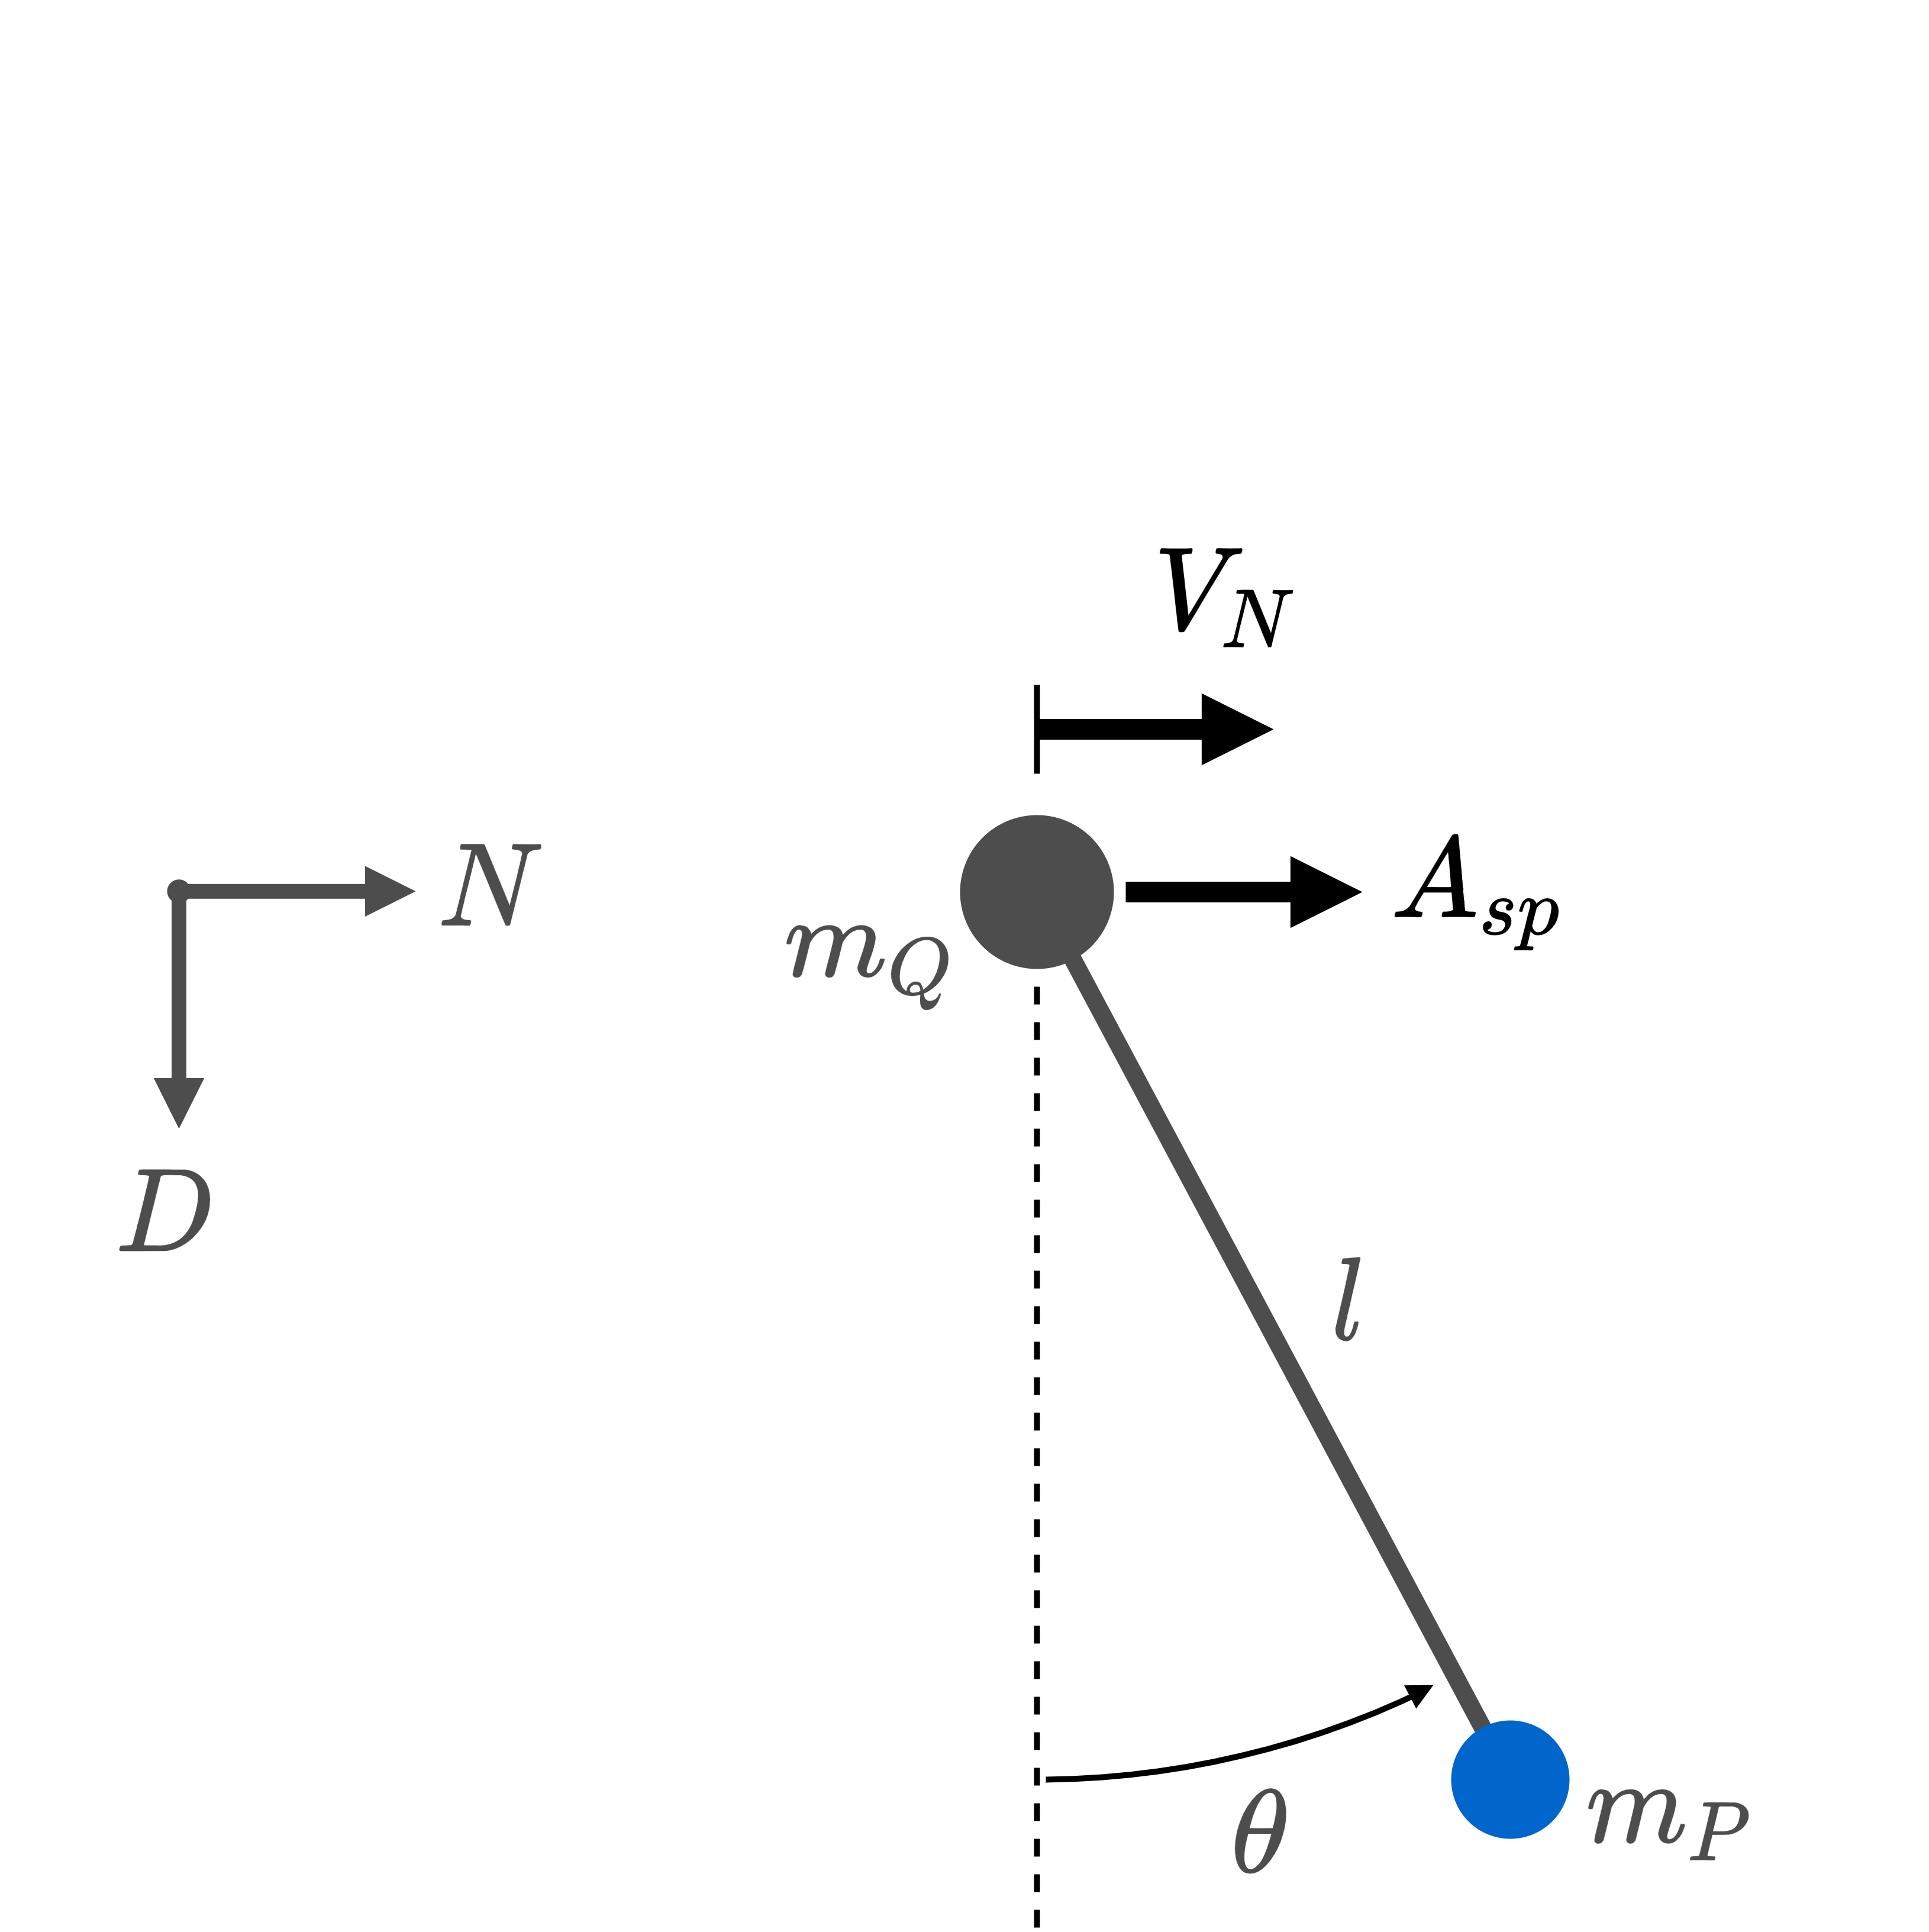
\includegraphics[width=0.45\linewidth]{floating_pend.png}            
        \caption{Floating pendulum model considered for system identification for a North velocity controller}
        \label{fig:floating_pend}
    \end{figure}

    \paragraph
    The considered LQR and MPC needs to control the North velocity of the quadrotor 
    and therefore has the input vector,
    \begin{equation}
        \bm{u} = \begin{bmatrix}
            A_{N,sp}
        \end{bmatrix} .
    \end{equation}
    The controllers require state feedback from the quadrotor and payload,
    hence the state vector of the considered plant is defined as,
    \begin{equation}
        \bm{x} = \begin{bmatrix}
            V_N & \theta & \dot{\theta}
        \end{bmatrix}^T .
    \end{equation}
    % This is the state vector of the considered plant, 
    % but the controllers apply an augmented state vector that will be discussed in Chapter~\ref{chap:control_systems}.
    Note that position is not included in the state vector because it does not affect the velocity controller.
    Also note that the inner loop controllers handle the attitude dynamics of the quadrotor.
    During pure longitudinal velocity setpoints the quadrotor experiences negligible altitude changes
    because of sufficient speed in the altitude controllers.
    The plant seen by the system identification process therefore mimics the common pendulum-on-a-cart model.
    A schematic of this 2D plant considered for system identification is shown in Figure \ref{fig:floating_pend}.
    In the following sections, simulations of the full quadrotor and payload system will be performed
    and different methods will be applied to identify models of this plant.
    % The differential equations that describe the motion of this system 
    % were derived with Lagrangian mechanics in Chapter~\ref{chap:modelling}. 

    % From this derivation it is clear that the angular velocity of the payload, $\dot{\theta}$, is required to described the system dynamics.
    % However, $\dot{\theta}$ is not measured directly on the considered practical quadrotor setup.
    % Instead, the payload angle, $\theta$, is measured by a potentiometer attached to a ADC on Honeybee as described in Chapter \ref{chap:system_overview}.
    % As expected, this measurement is extremely noisy.
    % \murray{Maybe insert figure to show noise}
    % % Figure \ref{} shows the angle measurement during a practical experiment of the payload while Honeybee is held stationary
    % Numerical differentiation is applied to the noisy $\theta$ signal which results in a very inaccurate estimation of $\dot{\theta}$.
    % Therefore it is desirable to rather use $\theta$ in the system identification process. 

